\exerciseset{In Exercises}{, a region is given. Find the area of the region using Simpson's Rule:
\begin{enumerate}
\item	[(a)] where the measurements are in centimeters, taken in 1 cm increments, and
\item	[(b)] where the measurements are in hundreds of yards, taken in 100 yd increments.
\end{enumerate}
}{

\exercise{\begin{minipage}{\linewidth}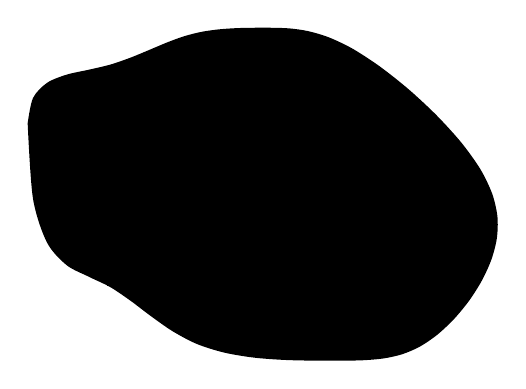
\begin{tikzpicture}[yscale=.6]

\draw [{\colorone},thick,fill={\coloronefill},smooth] plot coordinates {(0,2.)(0.06639,2.527)(0.2407,2.839)(0.4857,3.009)(0.7641,3.112)(1.039,
3.221)(1.294,3.367)(1.532,3.53)(1.759,3.689)(1.98,3.823)(2.2,3.915)(2.
42,3.967)(2.64,3.992)(2.86,4.)(3.08,4.)(3.305,3.987)(3.543,3.93)(3.
808,3.797)(4.107,3.558)(4.45,3.185)(4.815,2.703)(5.17,2.152)(5.483,1.
577)(5.723,1.018)(5.872,0.5022)(5.938,0.02083)(5.93,-0.4363)(5.861,-0.
88)(5.741,-1.319)(5.58,-1.742)(5.389,-2.128)(5.179,-2.456)(4.96,-2.
705)(4.737,-2.865)(4.502,-2.953)(4.243,-2.991)(3.95,-3.)(3.614,-2.999)
(3.244,-2.984)(2.86,-2.935)(2.484,-2.829)(2.137,-2.646)(1.832,-2.378)(
1.558,-2.06)(1.299,-1.734)(1.039,-1.443)(0.7641,-1.222)(0.4857,-0.
9779)(0.2407,-0.5015)(0.06639,0.4201)(0,2.)};

\draw (1,3.22) -- (1,-1.443) node [shift={(-3pt,0pt)},rotate=90,pos=.5] {\scriptsize 4.7};
\draw (2,3.823) -- (2,-2.5) node [shift={(-3pt,0pt)},rotate=90,pos=.5] {\scriptsize 6.3};
\draw (3,4) -- (3,-2.95) node [shift={(-3pt,0pt)},rotate=90,pos=.5] {\scriptsize 6.9};
\draw (4,3.62) -- (4,-3) node [shift={(-3pt,0pt)},rotate=90,pos=.5] {\scriptsize 6.6};
\draw (5,2.4) -- (5,-2.7) node [shift={(-3pt,0pt)},rotate=90,pos=.5] {\scriptsize 5.1};
\end{tikzpicture}
\end{minipage}}{\begin{enumerate}
\item		Area is $30.8667$ cm$^2$.
\item		Area is $308,667$ yd$^2$.
\end{enumerate}
}

\exercise{\begin{minipage}{\linewidth}
\begin{tikzpicture}[yscale=.6]

\draw [{\colorone},thick,fill={\coloronefill},smooth] plot coordinates {(0,1.)(0.05533,1.541)(0.2027,1.965)(0.414,2.278)(0.6613,2.483)(0.9167,
2.583)(1.157,2.588)(1.382,2.521)(1.595,2.409)(1.799,2.282)(2.,2.167)(
2.2,2.089)(2.4,2.068)(2.6,2.119)(2.8,2.257)(3.,2.5)(3.201,2.847)(3.
411,3.233)(3.636,3.58)(3.885,3.807)(4.167,3.833)(4.483,3.604)(4.815,3.
159)(5.139,2.561)(5.431,1.876)(5.667,1.167)(5.828,0.488)(5.917,-0.
1427)(5.943,-0.7173)(5.912,-1.228)(5.833,-1.667)(5.715,-2.028)(5.564,-
2.317)(5.389,-2.543)(5.199,-2.712)(5.,-2.833)(4.799,-2.912)(4.589,-2.
943)(4.364,-2.917)(4.115,-2.828)(3.833,-2.667)(3.513,-2.432)(3.153,-2.
149)(2.753,-1.851)(2.313,-1.568)(1.833,-1.333)(1.323,-1.155)(0.828,-0.
944)(0.4053,-0.5893)(0.1107,0.02133)(0,1)};

\draw (1,2.6) -- (1,-1.) node [shift={(-3pt,0pt)},rotate=90,pos=.5] {\scriptsize 3.6};
\draw (2,2.167) -- (2,-1.43) node [shift={(-3pt,0pt)},rotate=90,pos=.5] {\scriptsize 3.6};
\draw (3,2.5) -- (3,-2) node [shift={(-3pt,0pt)},rotate=90,pos=.5] {\scriptsize 4.5};
\draw (4,3.8) -- (4,-2.75) node [shift={(-3pt,0pt)},rotate=90,pos=.5] {\scriptsize 6.6};
\draw (5,2.8) -- (5,-2.83) node [shift={(-3pt,0pt)},rotate=90,pos=.5] {\scriptsize 5.6};
\end{tikzpicture}
\end{minipage}
}{\begin{enumerate}
\item		Area is 25.0667 cm$^2$
\item		Area is 250,667 yd$^2$
\end{enumerate}
}

}
